
\begin{frame}{Setup}
	\centering
	\begin{tikzpicture}
		\node[] (task) at (-6,1) {
			\begin{tikzpicture}
				\node[] (p) at (0,2) {\textbf{Planning Task}};
				\node[] (r1) at (0,-0.3) {
\includegraphics[scale=0.06]{images/rover1.png}};
				\node[] (r2) at (1.5,-0.3) {
\includegraphics[scale=0.06]{images/rover2.png}};
				\node[] (i1) at (-0.5,1) {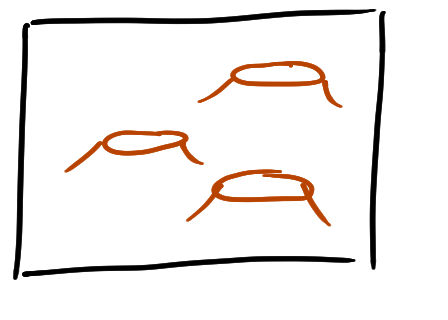
\includegraphics[scale=0.07]{images/image1.png}};
				\node[] (i2) at (0.5,1) {
\includegraphics[scale=0.07]{images/image2.png}};
				\node[] (i3) at (1.7,1) {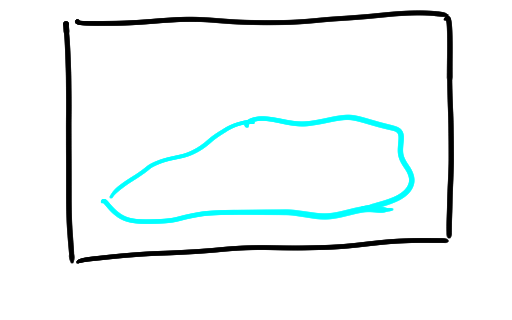
\includegraphics[scale=0.07]{images/image3.png}};
			\end{tikzpicture}
		};
	\node[] (p) at (0,2.5) {\textbf{Plans}};
	\node[draw, minimum height=3.5cm, minimum width=3cm, fill=white] (p3) at (0.4,0.4) {};
	\node[draw, minimum height=3.5cm, minimum width=3cm, fill=white] (p2) at (0.2,0.2) {};
	\node[draw, align=left, fill=white] (p1) at (0,0) {
			$drive(R_1,L_1,L2)$\\
			$takeImage_1(R_1)$\\
			$drive(R_2,L_4,L_5)$\\
			$takeImage_3(R_2)$\\
			$drive(R_2,L_5,L_6)$\\
			$\cdots$
	};
	\visible<2->{
		\node[] (hw) at (-4,-2.5) {
\includegraphics[scale=0.2]{images/human_why.png}};
	}
	\end{tikzpicture}

\end{frame}



\begin{frame}{Plan Property}
\centering
\begin{tikzpicture}
		\node[] (p1) at (-0.5,-3.0) {\samerover{1}{2}};
		\node[] (p2) at (3,-3.0) {\orderprop{1}{2}};
		\node[] (p3) at (6.5,-3.0) {\energylimit{1}};
		\node[] (p4) at (-0.5,0) {\specificrover{1}{2}};
		\node[] (p5) at (3,0) {\useconnection{1}{x}{y}};
		\node[] (p6) at (6.5,0) {\dontuseconnection{1}{x}{y}};
\end{tikzpicture}
\visible<2->{
	\rule{\textwidth}{0.05cm}
	\Large
	partial function p: $\cal{T} \times \cal{P}$$ ~\mapsto \{true, false\}$
}

\end{frame}



\begin{frame}{$\plans$-Entailment}
\centering
\begin{tikzpicture}
	\node[draw, minimum width=2.0cm, minimum height=0.6cm, inner sep=0pt] at (0,-2.2) {
		\begin{tikzpicture}
			\node[align=center] (kb) at (0,0) {knowledge base\\ task and set of plans $\Pi$};	
			\node[] (i1) at (-4.6,0) {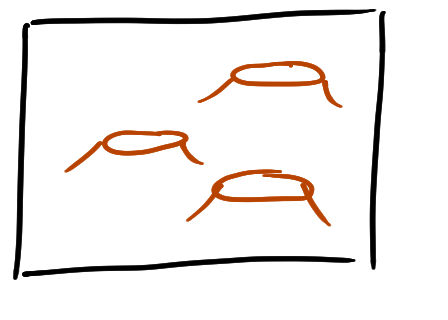
\includegraphics[scale=0.06]{images/image1.png}};
			\node[] (i2) at (-3.6,0) {
\includegraphics[scale=0.06]{images/image2.png}};
			\node[] (i3) at (-2.6,0) {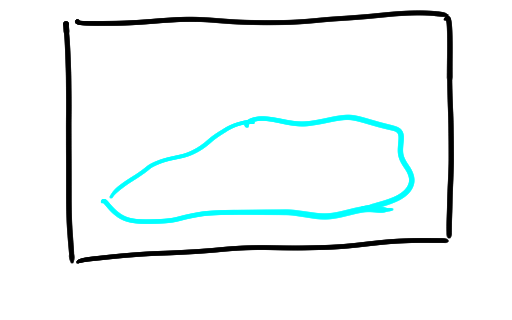
\includegraphics[scale=0.06]{images/image3.png}};

			\node[] (r1) at (2.9,0) {
\includegraphics[scale=0.04]{images/rover1.png}};
			\node[] (r2) at (3.9,0) {
\includegraphics[scale=0.04]{images/rover2.png}};
		\end{tikzpicture}	
	};

	\node[draw, align=center, inner sep=1pt] (P1) at (3,0.5) {
		\specificrover{1}{1}
	};
	\node[] (no) at (2.9,1.4) {
\includegraphics[scale=0.1]{images/no.png}}; 
	%\node[] (P1n) at (3,0.5) {
	%	
\includegraphics[scale=0.3]{images/no.png}
	%};
	\node[draw, align=center, inner sep=1pt] (P4) at (-3,0.5) {
		\dontuseconnection{1}{1}{2}
	};

	\visible<2->{
		%\draw[thick, ->] (P2) to (P3);
		\draw[thick, ->, line width=0.05cm] (P4) to node[above] {$\plans$-entails} (P1);
	}

\end{tikzpicture}

\visible<3->{
	\rule{\textwidth}{0.05cm}
	\Large
	$p$ $\Pi$-entails q: $\modelsof{\plans}{\prop} \subseteq \modelsof{\plans}{\propq}$
	$\modelsof{\plans}{\prop} := \{\plan \mid \plan \in \plans, \plan \models \prop\} $	
}

\end{frame}



\begin{frame}{Plan Space Explanation}
\centering
\begin{tikzpicture}
	\visible<3->{
	\node[] (p) at (4,3.5) {
		\resizebox{!}{1.5cm}{%
		\begin{tikzpicture}
			\node[draw, inner sep=1pt] (p1) at (0,0) {
				\dontuseconnection{1}{1}{2}
			};
			\node[draw, inner sep=1pt] (p2) at (5,0) {
				\specificrover{1}{1}
			};
			\node[] (no) at (5,0.9) {
\includegraphics[scale=0.1]{images/no.png}}; 
			\draw[thick, ->] (p1) to (p2);
		\end{tikzpicture}
		}
	};
	}

	\node[] (task) at (0,-1) {
		\resizebox{!}{5cm}{%
		\begin{tikzpicture}
			\node[] (t) at (1.5,2) {
\includegraphics[scale=0.07]{images/rover2.png}};
			\node[] (t) at (-5,-2.5) {
\includegraphics[scale=0.07]{images/rover1.png}};

			\node[] (m) at (0,0) {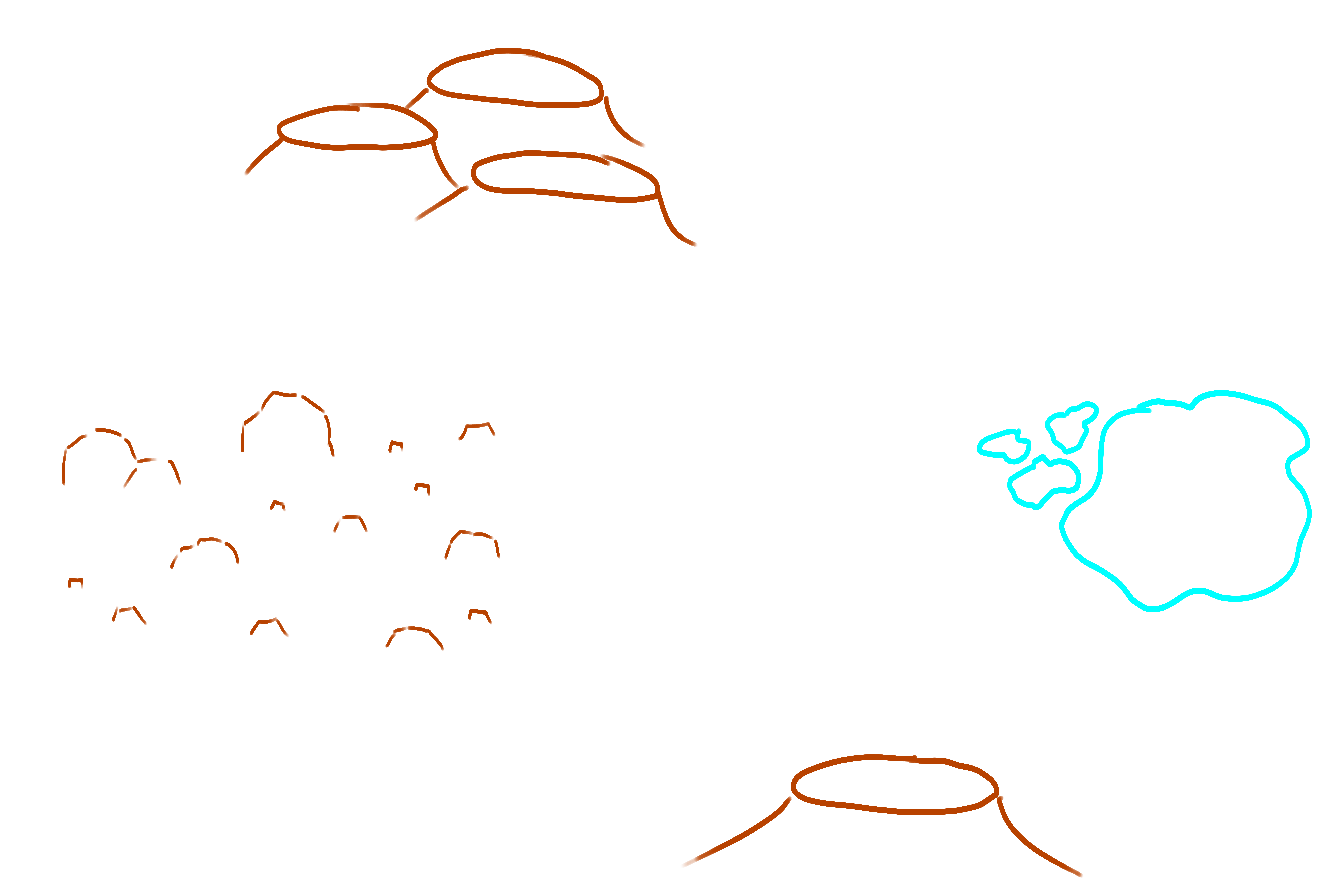
\includegraphics[scale=0.2]{images/mars_new.png}};

			\node[draw, circle, inner sep=3pt] (l1) at (-3,-3) {$L_1$};
			\node[draw, circle, inner sep=3pt] (l2) at (-2.1,1.3) {$L_2$};
			\node[draw, circle, inner sep=3pt] (l3) at (-0.5,-1) {$L_3$};
			\node[draw, circle, inner sep=3pt] (l4) at (3,2) {$L_4$};
			\node[draw, circle, inner sep=3pt] (l5) at (1.8,0) {$L_5$};
			\node[draw, circle, inner sep=3pt] (l6) at (3.2,-2.5) {$L_6$};

			\draw[thick] (l1) to (l2);
			\draw[thick] (l1) to (l3);
			\draw[thick] (l2) to (l3);
			\draw[thick] (l3) to (l5);
			\draw[thick] (l4) to (l5);
			\draw[thick] (l4) to (l6);
			\draw[thick] (l5) to (l6);
			\visible<2->{
				\draw[thick, red, ->, line width=0.1cm] (l1) to (l2);
				\draw[thick, mLightGreen, ->, line width=0.1cm] (l1) to (l3);
				\draw[thick, mLightGreen, ->, line width=0.1cm] (l3) to (l2);
			}

			\node[] (g) at (-1.9,-4) {\Large \textbf{goal}:};
			\node[] (i1) at (-0.5,-4) {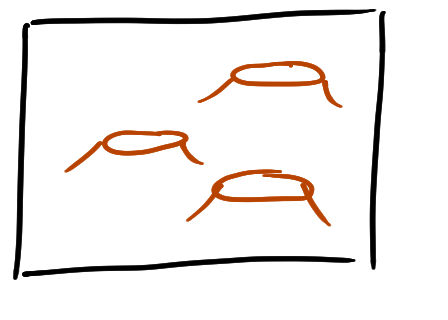
\includegraphics[scale=0.1]{images/image1.png}};
			\node[] (i2) at (0.8,-4) {
\includegraphics[scale=0.1]{images/image2.png}};
			\node[] (i3) at (2.5,-4) {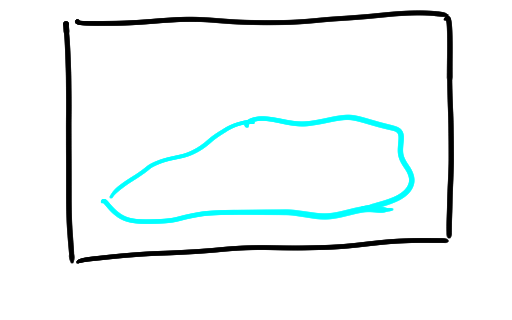
\includegraphics[scale=0.1]{images/image3.png}};
		\end{tikzpicture}
		}
	};


	\node[] (human_why) at (-4,1.5) {
\includegraphics[scale=0.2]{images/human_why.png}};
	\node[] (ai_exp) at (4,1.5) {
\includegraphics[scale=0.2]{images/ai_exp.png}};


		\node[draw, align=left, fill=white] (plan) at (-1,3) {
				\scriptsize
				$drive(R_1,L_1,L2)$\\[-0.2cm]
				\scriptsize
				$takeImage_1(R_1)$\\[-0.2cm]
				\scriptsize
				$drive(R_2,L_4,L_5)$\\[-0.2cm]
				\scriptsize
				$takeImage_3(R_2)$\\[-0.2cm]
				\scriptsize
				$drive(R_2,L_5,L_6)$\\[-0.2cm]
				\scriptsize
				$\cdots$
		};

\end{tikzpicture}

\end{frame}





